\documentclass[twoside,a4paper]{book}
\usepackage{graphicx}
\usepackage{hyperref}
\usepackage{amsmath}
\usepackage{amssymb}
\usepackage{textcomp}
\usepackage[utf8]{inputenc}
\usepackage[polish]{babel}
\usepackage[T1]{fontenc}
\usepackage{standalone}
\usepackage{array}
% pakiet stosowany do url'i w bibliografii, zamienia odnośniki na ładnie sformatowane
\usepackage{url}
% pakiety służące do numerowania i tworzenia algorytmów
\usepackage{algorithmic}
\usepackage{algorithm}
% redefinicja etykiety nagłówkowej listy algorytmów, domyślna jest po angielsku
\renewcommand{\listalgorithmname}{Spis algorytmów}

\usepackage[section]{placeins}
\usepackage{pdfpages}

% pakiet do wyliczania skali, przydatny przy dużych obrazkach
\usepackage{pgf}
% pakiet służący do automatycznego sortowania odnośników do bibliografii
\usepackage[sort]{natbib}
% tworzenie listingów
\usepackage{listings}
% tworzenie figur wewnątrz figur
\usepackage{subfig}
% do automatycznego skracania nazw rozdziałów i podrozdziałów używanych w nagłówkach strony by mieściły się w jednej linii
\usepackage[fit]{truncate}
% fancyhdr - ładne nagłówki, definicja wyglądu nagłówka, numery stron będą umieszczane w nagłówku po odpowiedniej stronie
\usepackage{fancyhdr}
\pagestyle{fancy}
\renewcommand{\chaptermark}[1]{\markboth{#1}{}}
\renewcommand{\sectionmark}[1]{\markright{\thesection\ #1}}



\fancyhf{}
\fancyhead[LE,RO]{\bfseries\thepage}
% tutaj ograniczamy szerokość pola w nagłówku zawierającego nazwę rozdziału/podrozdziału do 95% szerokości strony
% redefinicja sposobu prezentacji nazw domyślnie wypisywanych wielkimi literami (np. domyślnie w nagłówku Spis treści będzie miał postać SPIS TREŚCI)
% Uwaga! to może popsuć wielkie litery w ogóle! Jak coś nie działa należy usunąć \nouppercase{} z poniższych definicji
\fancyhead[LO]{\nouppercase{\bfseries{\truncate{.95\headwidth}{\rightmark}}}}
\fancyhead[RE]{\nouppercase{\bfseries{\truncate{.95\headwidth}{\leftmark}}}}
\renewcommand{\headrulewidth}{0.5pt}
\renewcommand{\footrulewidth}{0pt}

% definicja typu prostego wymagana przez pierwsze strony rozdziałów itp.
% powyższe reguły niestety tych stron nie dotyczą, gdyż Latex automatycznie przełącza je pomiędzy fancy a plain
% w tym wypadku eliminujemy nagłówki i stopki na stronach początkowych
\fancypagestyle{plain}{%
 \fancyhead{}
 \fancyfoot{}
 \renewcommand{\headrulewidth}{0pt}
 \renewcommand{\footrulewidth}{0pt}
}

\parskip 0.05in


% makro umożliwiające otaczanie symboli okręgami
\usepackage{tikz}
% brak justowania tekstu (bazą okręgu będzie linia tekstu)
\newcommand*\mycirc[1]{%
  \begin{tikzpicture}
    \node[draw,circle,inner sep=1pt] {#1};
  \end{tikzpicture}}

% pionowe justowanie tekstu, środek okręgu pokrywa się ze środkiem tekstu
\newcommand*\mycircalign[1]{%
  \begin{tikzpicture}[baseline=(C.base)]
    \node[draw,circle,inner sep=1pt](C) {#1};
  \end{tikzpicture}}

% zmiana nazwy twierdzeń i lematów
\newtheorem{theorem}{Twierdzenie}[section]
\newtheorem{lemma}[theorem]{Lemat}

% tworzenie definicji dowodu
\newenvironment{proof}[1][Dowód]{\begin{trivlist}
\item[\hskip \labelsep {\bfseries #1}]}{\end{trivlist}}
% \newenvironment{definition}[1][Definicja]{\begin{trivlist}
% \item[\hskip \labelsep {\bfseries #1}]}{\end{trivlist}}
% \newenvironment{example}[1][Przykład]{\begin{trivlist}
% \item[\hskip \labelsep {\bfseries #1}]}{\end{trivlist}}
% \newenvironment{remark}[1][Uwaga]{\begin{trivlist}
% \item[\hskip \labelsep {\bfseries #1}]}{\end{trivlist}}

% definicja czarnego prostokąta zwyczajowo dodawanego na koniec dowodu
\newcommand{\qed}{\nobreak \ifvmode \relax \else
      \ifdim\lastskip<1.5em \hskip-\lastskip
      \hskip1.5em plus0em minus0.5em \fi \nobreak
      \vrule height0.75em width0.5em depth0.25em\fi}

% poniższymi instrukcjami można sterować co ma być numerowane a co nie i co ma być wyświetlane w spisie treści
% \setcounter{secnumdepth}{3}
% \setcounter{tocdepth}{5}

% definicja czcionki mniejszej niż tiny (domyślnie takiej małej nie ma)
\usepackage{lmodern}
\makeatletter
  \newcommand\tinyv{\@setfontsize\tinyv{4pt}{6}}
\makeatother

% definicja jeszcze mniejszej czcionki
\usepackage{lmodern}
\makeatletter
  \newcommand\tinyvv{\@setfontsize\tinyvv{3.5pt}{6}}
\makeatother

% pakiet do obsługi wielostronicowych tabel
\usepackage{longtable}
\setlength{\LTcapwidth}{\textwidth}

\usepackage[section] {placeins}


\usepackage{multirow}

\usepackage{slantsc}
\usepackage[labelsep=endash]{caption}
\addto\captionspolish{\renewcommand{\figurename}{Rys.}}
\addto\captionspolish{\renewcommand{\tablename}{Tab.}}
\addto\captionspolish{\renewcommand*{\appendixpagename}{Dodatki}}
\addto\captionspolish{\renewcommand*{\appendixtocname}{Dodatki}}
\addto\captionspolish{\renewcommand*{\appendixname}{Dodatek}}

\setcounter{secnumdepth}{5}

\usepackage[toc,page]{appendix}

\begin{document}

\chapter{Analiza projektowa}
Rozdział poświęcony analizie wybranych technologii oraz wymagań projektu. Przedstawiono również wstępną analizę dotyczącą przypadków użycia oraz metod testowania produktu.
\section{Wybrane technologie}
Krótki opis teoretyczny wybranych technologii - C++ oraz bibliotek QT. 

\subsection{QT}

QT jest zespołem przenośnych bibliotek oraz narzędzi programistycznych stworzonych w C++ do tworzenia aplikacji desktopowych, zagnieżdżonych, jak również mobilnych. Wspiera systemy takie jak: Linux, OS X, Widows, xWorks, QNX, Android, iOS, BlackBerry, Sailfish OS, dzięki czemu jest nadzwyczaj uniwersalnym narzędziem kompatybilnym z następującymi językami programowania: C++, QML (QT Modeling Language), Python, Ring, Go, Rust, PHP i Java.~\cite{qtAbout}~\cite{qtLang}\\
QT zapewnia listę dodatkowych możliwości rozszerzających C++. Są to między innymi: \\
- mechanizmy pozwalające na komunikację między obiektami zwane sygnałami i otworami (slots)\\
- wyjątkowa możliwość edycji wyglądu i responsywności obiektów \\
- swobodna możliwość edycji zachowań w przypadku różnego rodzaju zdarzeń \\
- kontekstowe tłumaczenie stringów do internacjonalizacji\\
- hierarchiczne i responsywne drzewa obiektowe, organizujące strukturę obiektów\\
- automatyczna zmiana wartości wskaźników na 0 w przypadku zniszczenia obiektu, w przeciwieństwie do wskaźników w C++, które stając się zawieszonymi (dangling pointers) 
~\cite{qtLang}
\subsection{C++}

C++ jest powszechnie stosowanym językiem programistycznym, będącym potomkiem języka C, w którym wprowadzono szereg udogodnień.W porównaniu z C, C++ zapewnia dokładniejsze sprawdzanie typów danych, wspiera abstrakcje, programowanie obiektowe (z tego względu mówi się o nim jako o języku pseudo-obiektowym), programowanie uogólnione i więcej styli programistycznych. Do wspieranych założeń programowania obiektowego należą polimorfizm, enkapsulacja i dziedziczenie.Nowsza wersja C posiada również bardzo dużą ilość bibliotek, których wykorzystanie znacznie ułatwia jego wykorzystanie.

\section{Architektura systemu}
System składa się z warstwy aplikacji oraz warstwy transportowej. Komunikacja zrealizowana jest za pomocą broadcastu przy pomocy protokołu UDP (user data protocol). 

\subsection{Architektura aplikacji}
Aplikację zrealizowano w wyżej wymienionym języku C++ z wykorzystaniem wielu bibliotek QT np. QWidget, QString, QtGui,QPainter itd.. Do funkcji auto uzupełniania tekstu posłużono się algorytmem wykorzystującym skompresowane drzewo trie. 
\subsubsection{Sompresowane Drzewo Trie}
Drzewo Trie jest drzewem służącym docelowo do sortowania wartości tesktowego typu danych, w którym każdemu węzłowi przypisany jest  wspólny prefix(fragment klucza). Wartości tekstowe zapisywane są w liściach drzewa. ~\citep{trieTree}
Do drzewa wczytywane zostają wszystkie słowa z danego mu słownika, a następnie każde rozkłada się na litery i rozmieszcza w drzewie, tak by czytając znaki od korzenia do liścia tworzyły pożądany ciąg. Biorą na przykład słownik składający się z następujących słów: mak, róża, kolec, małż, koc, moher otrzymujemy następujące drzewo ~\ref{fig:trie}.
\begin{figure}[!h]
		\centering
		\scalebox{.7}{
		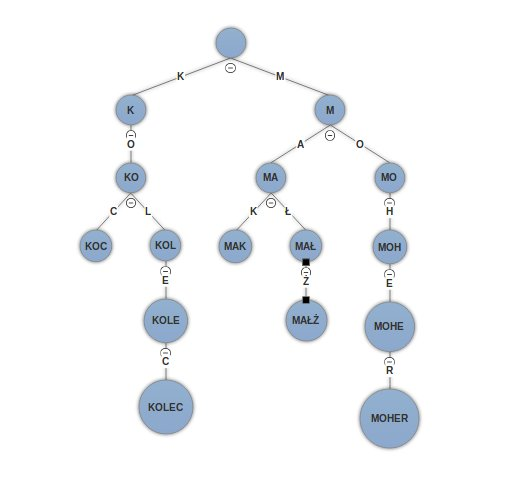
\includegraphics[width=0.7\textwidth]{img/trie.jpg}}
		\caption{Przykładowe drzewo typu Trie. }
		\label{fig:trie}
\end{figure}
W ten sposób poszukując słów zaczynających się na ''ko'' w bardzo prosty sposób możemy określić, że zaliczają się do nich koc oraz kolec. 
Drzewo to w znaczący sposób skraca czas przeszukiwania dużych słowników (w wypadku tego projektu 3639970 wyrazów) i umożliwia np. auto uzupełnianie albo korektę słów bieżąco wpisywanych przez użytkownika.

Zastosowany algorytm wykorzystuje fakt występowania wspólnych węzłów i zapamiętuje jedynie numer ostatniego węzła związanego z wyszukiwanym słowem np. dla frazy ''ko
'' - węzeł nr. 2, a następnie pobiera wartości wszystkich dzieci tego węzła, zespala je i tworzy wszystkie możliwe końcówki (tu ''c'' oraz ''lec''), które w połączeniu z szukaną frazą dają "auto uzupełniane" słowa.
\subsection{Komunikacja aplikacji}
System umożliwia komunikację poprzez broadcast z innymi użytkownikami jak i poprzez specjalne API Google z przeglądarką internetową. 

Broadcast jest metodą komunikacji (rozsyłania danych) między jednym nadawcą, a wieloma odbiorcami w tym samym czasie. Jest to dyfuzyjny, jednokierunkowy tryb  transmisji charakterystyczny dla sieci LAN. Protokołem regulującym dany ruch sieciowy jest w tym wypadku UDP (User Datagram Protocol). Jest to bezpołączeniowy protokół, który pozwala aplikacjom dobudować własne - niezbędne do poprawnego działania, protokoły. 
Zapewnia on aplikacji możliwość wysyłania enkapsulowanych datagramów IP bez potrzeby wytworzenia połączenia, co jest jednocześnie dużo szybszą metodą komunikacji, niż tryb synchroniczny. Nie dba on o to, czy wysłane ramki dotrą do odbiorcy w całości, co jest typowe dla komunikacji asynchronicznej.
UDP transmituje segmenty złożone z 8-bajtowego nagłówka oraz fragment przesyłanych danych, będący formą wiadomości. 
UDP zapewnia informację o portach źródłowych i docelowych. 
Port źródłowy jest przydatny w momencie, gdy urządzenie odbiorcy zechce odesłać odpowiedź na otrzymany segment.
Rozmiar ramki wynosi od 8-65 515 bajtów. ~\cite{UDP}

Google Custom Search umożliwia stworzenie własnej wyszukiwarki umożliwiającej na przeszukiwanie zarówno stron internetowych jak i obrazów. Możliwe jest zawężenie i personalizacja wyników wyszukiwania np. do wyników pochodzących z konkretnej strony, lub zawierających sprecyzowaną frazę.  Google Seachr Engine występuje w dwóch wersjach - Custom Search Engine, która jest darmowa oraz Google Site Search, które jest werjsą płatną. Do potrzeb projektowych wystraczająca jest wersja darmowa, która umożliwia korzytsanie z dodatkowych API umożliwiających zwrócenie wyników wyszukiwania w postaci pliku XML czy też JSON. API te upraszaczją komunikację aplikacji z przeglądarką do zapytań RESTowych typu get w celu otrzymania uporządkowanej struktury danych. ~\cite{googleAPI}


 
\section{Wymagania funkcjonalne}
Po przeanalizowaniu problemu klawiatury ekranowej oraz potrzeb osób chorych na ALS stwierdzono następujące wymanagania funkcjonalne:
\begin{itemize}
\item Klawiatura ekranowa reagująca na sygnał wejściowy będący współrzędnymi punktu fiksacji, które określane są z dokładnością jednego stopnia. Zakładając, że odległość użytkownika od ekranu to 60cm, wyliczono iż dokładność wyznaczania pozycji to obszar ok. 3,2 cm powierzchnii ekranowej. Dla komputera o ekranie 14 cal (monitor testowy), gdzie rozmiar pojedzyńczego piksela to ok. 0,2269 mm - to, w przybliżeniu, 141px dla każdego przycisku. 
\item Możliwość auto uzupełniania słów za pomocą słownika języka polskiego.
\item Możliwość wprowadzenia przycisków w stan nieaktywny. 
\item Wykorzytstywanie polskich znaków w tekście. 
\item Wysyłanie wiadomości za pomocą broadcastu. 
\item Wyszukiwanie stron w przeglądarce Google.
\item Możliwość konfugurowania wyglądu aplikacji - różne stopnie kontrastu oraz kolorystyki, a także rozmiaru czcionki tekstu wpisywanego. 
\end{itemize}
Szczegółowe przypadki użycia klawiatry zobrazowano w rozdziale "Przypadki użycia"~\ref{sec:uml}.

\subsection{Przypadki użycia}
  \label{sec:uml}
  Na zamieszczonym rysunku ~\ref{fig:useCase} przedstawiono diagram przypadków użycia przedstawiający możliwe interakcje użytkownika z aplikacją. 
\begin{figure}[!h]
		\centering
		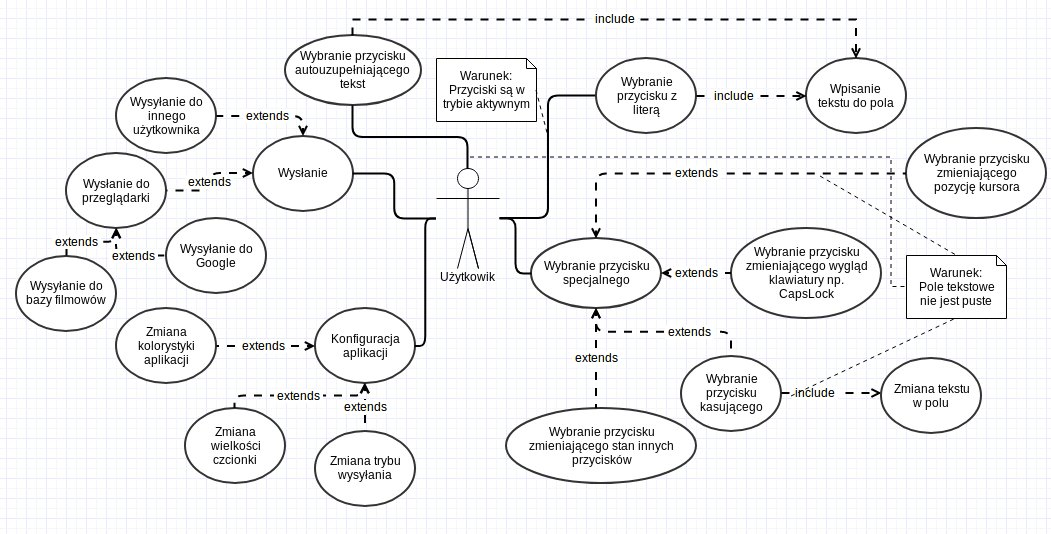
\includegraphics[scale=0.4]{img/useCase.jpg}
		\caption{Wykres przypadków użycia stworzony za pomocą strony Gliffy.com}
		\label{fig:useCase}
\end{figure}

Aby rozpocząć pracę z klawiaturą należy odblokować pisanie znaków wybirając przycisk ''start''.
Gówną funkcjonalnością, a zarazem najczęściej zachodzącym przypadkiem użycia będzie wybór przycisku z literą w celu wypisania tekstu na ekranie. Użytkownik ma do wyboru klawiaturę podstawową z 28 znakami oraz cyframi z zakresu 0-9 oraz 2 tablice przycisków ze znakami specjalnymi oraz jedną poświęconą jedynie polskim znakom. Każdy z przycisków reaguje na zmianę położenia punktu fiksacji - w momencie, w którym wykryte zostanie położenie nad przyciskiem naliczany zostaje czas, którego narastanie wizualizuję się za pomocą pasku postępu. Gdy 100\% postępu zostanie osiągnięte dana litera pojawia się na ekranie w przeznaczonym obszarze i w określonej, za pomocą kursora, pozycji w tekście. W przypadku jeśli użytkownik zechce zmienić wielkość liter może wybrać między opcją CapsLock (stałym powiększeniem liter wpisywanych), bądź Shift (zwiększającym kolejną literę dodaną do tekstu, następnie zmieniając wielkość liter na małe). W obu wypadkach następuję zmiana wyglądu całej klawiatury. 
Po tekście można poruszać się za pomocą strzałek - ruch w prawo (do początku tekstu) i lewo (na koniec tekstu) o jeden znak, lub specjalnych przycisków ''home'' oraz ''end'', które przenoszą kursor odpowiednio na początek i koniec tekstu. Przyciski Enter oraz Spacja traktowane jako zwykłe znaki. Fiksacja na przycisku Backspace usuwa ostatni wpisany znak, a   na przycisku ''czyść'' usunięcie wszystkiego co znajduje się w polu tekstowym. Wyróżnia się też innego rodzaju przyciski specjalne, zmieniające wygląd klawiatury - są to przyciski do znaków specjalnych oraz polskich liter. Pierwszy z wymienionych w pierwszym kroku prezentuje wszystkie znaki specjalne powszechnego użytku np. wykrzyknik, cudzysłów, średnik, a przy powtórnym wciśnięciu na klawiaturze pojawiają się popularne emotikony, które znalazły tam swoje miejsce, ze względu na możliwość wysyłania wiadomośći do innych użytkowników i mają za zadanie ułatwienie reprezentacji emocjonalego przekazu wiadomości. W przypadku gdy użytkownik wpisał już jakiś fragment tekstu możę posłużyć się przyciskiem podpowiedzi, które działają na zasadzie auto uzupełniania tekstu na podstawie słów znalezionych w słowniku. Aby zmienić wygląd aplikacji lub tryb wysyłania należy skorzytać z przycisku menu. To pozwoli na wybranie schematu kolorstycznego aplikacji oraz na dobór wilekości czcionki. Użytkownik może wybrać również jeden z trzech trybów rozsyłania zapisanego przez niego tekstu - są to: Google Search, Filmweb oraz Broadcast (w celu czatu). W zależności od wybranego trybu, przycisk ''wyślij'' powoduje wywołanie odpowiedniej akcji.
\section{Propozycja rozwiązania}
\subsection{Zakres projektu}

\subsection{Interfejs oprogramownia}
\begin{figure}[!h]
		\centering
		\scalebox{.9}{
		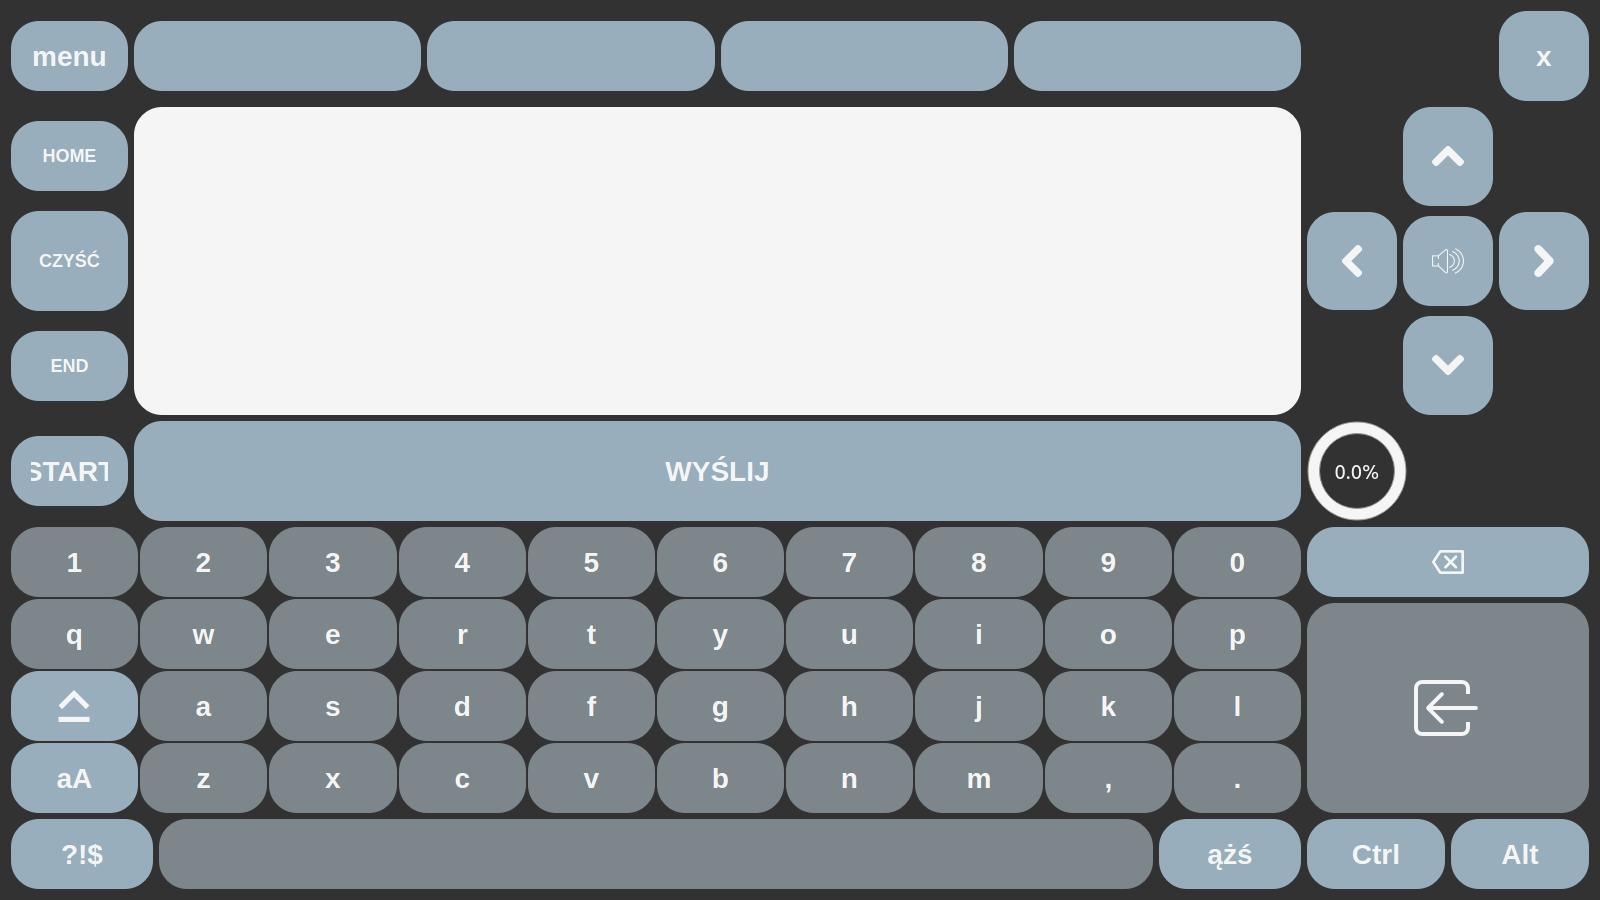
\includegraphics[width=1\textwidth]{img/mainInactive.jpg}}
		\caption{Początkowy wygląd aplikacji z nieaktywnymi przyciskami. }
		\label{fig:inactive}
\end{figure}
\begin{figure}[!h]
		\centering
		\scalebox{.9}{
		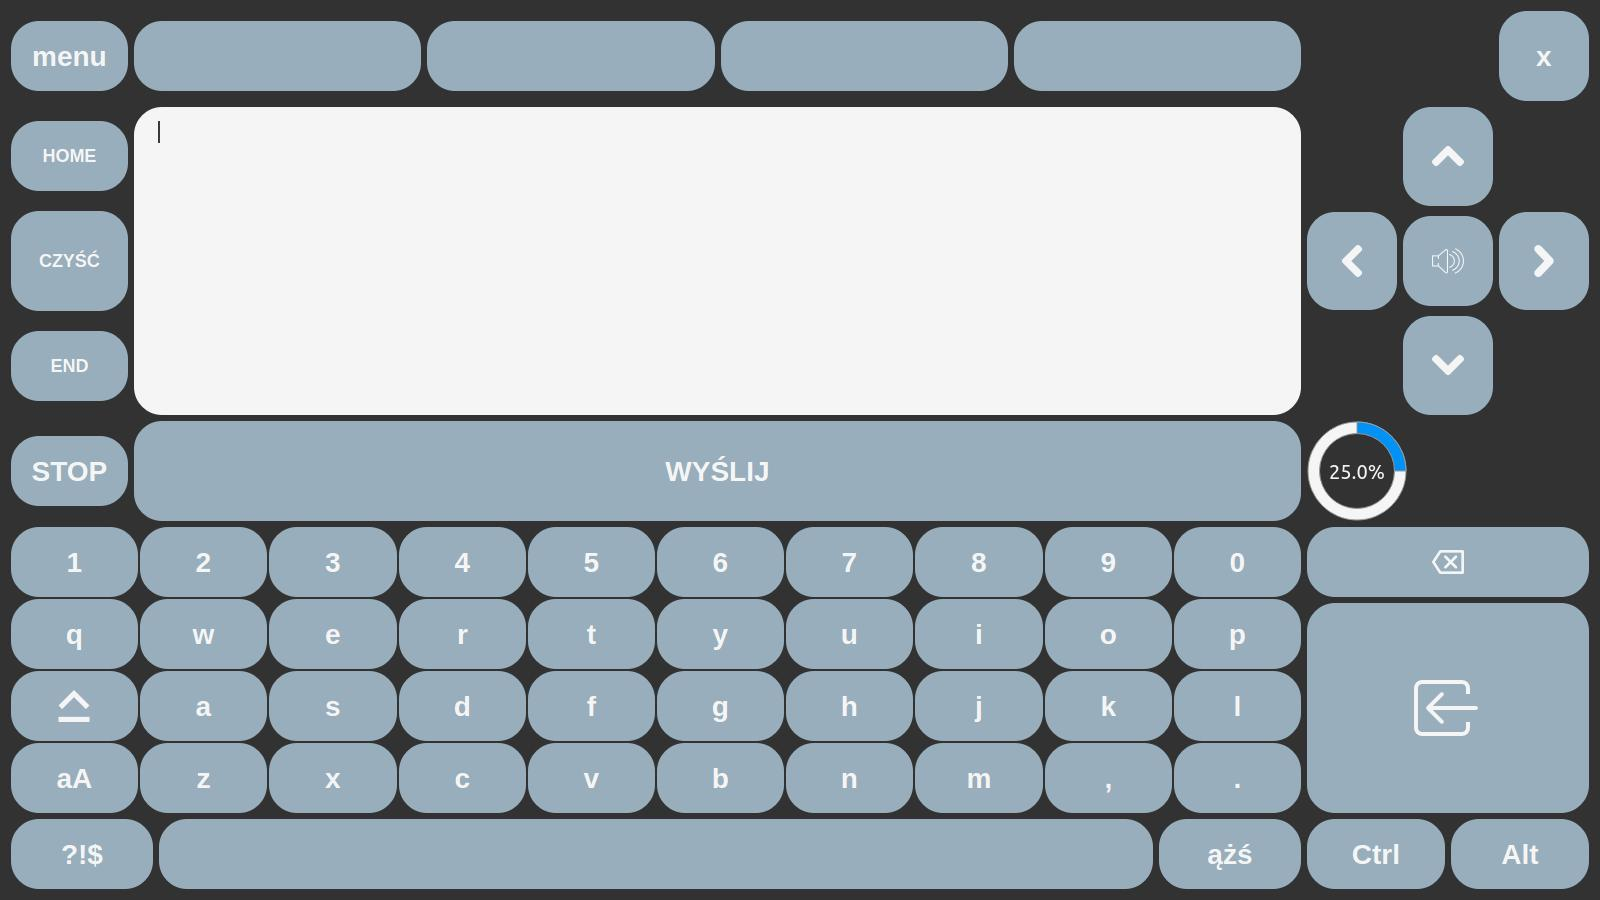
\includegraphics[width=1\textwidth]{img/mainActive.jpg}}
		\caption{Aktywny wygląd aplikacji. }
		\label{fig:active}
\end{figure}
\begin{figure}[!h]
		\centering
		\scalebox{.9}{
		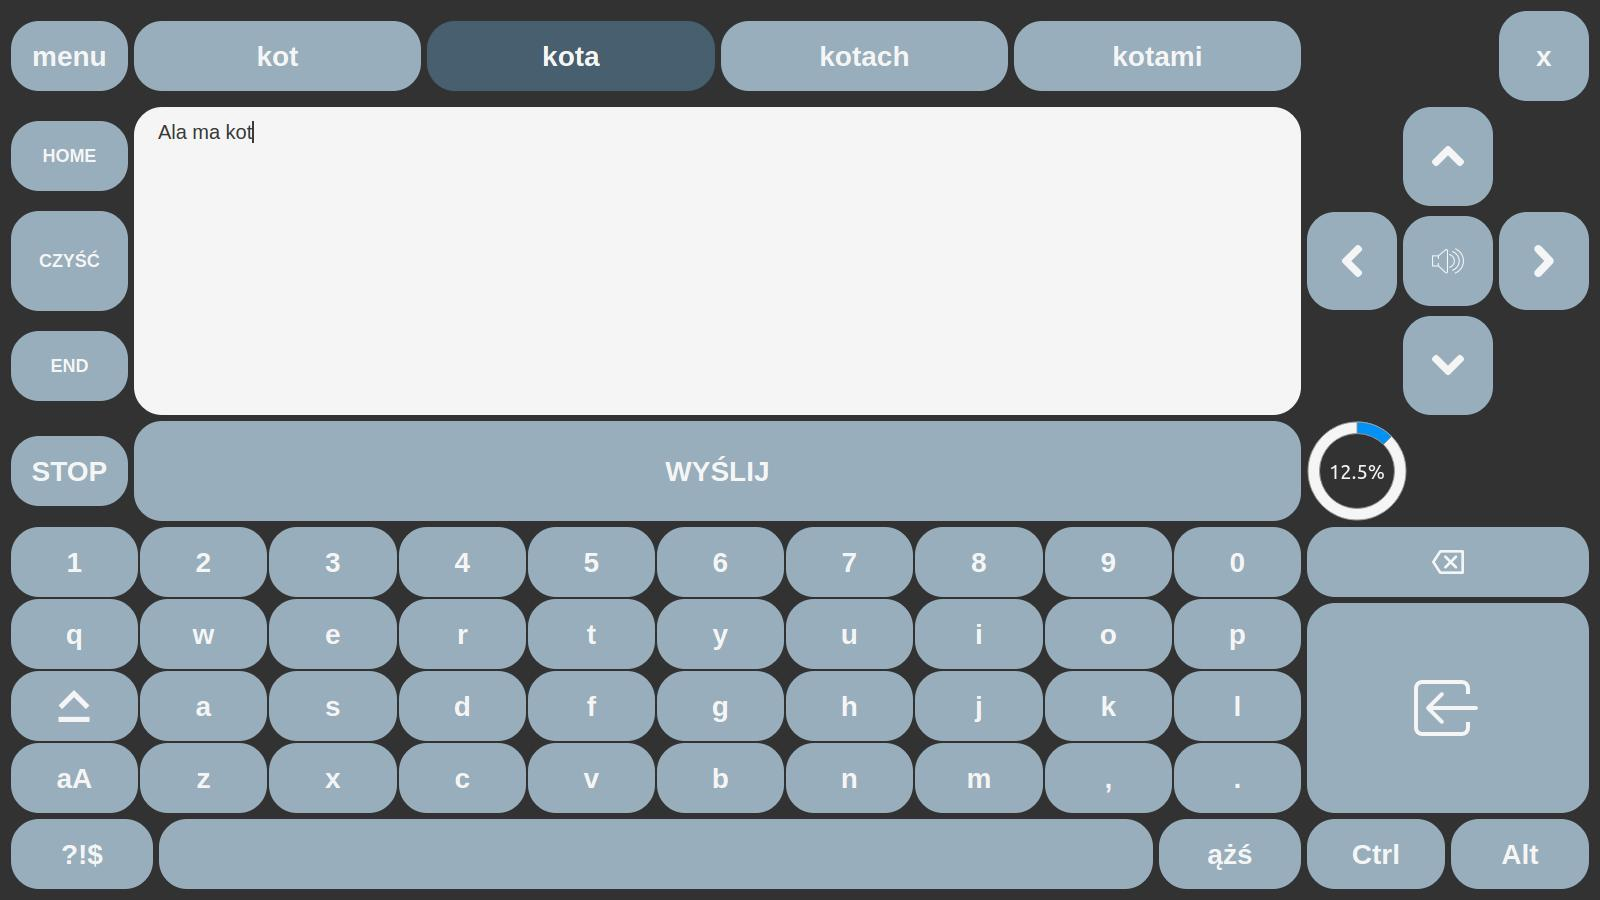
\includegraphics[width=1\textwidth]{img/auto.jpg}}
		\caption{Przykład wyświetlanych opcji autouzupełniania. }
		\label{fig:auto}
\end{figure}
\begin{figure}[!h]
		\centering
		\scalebox{.9}{
		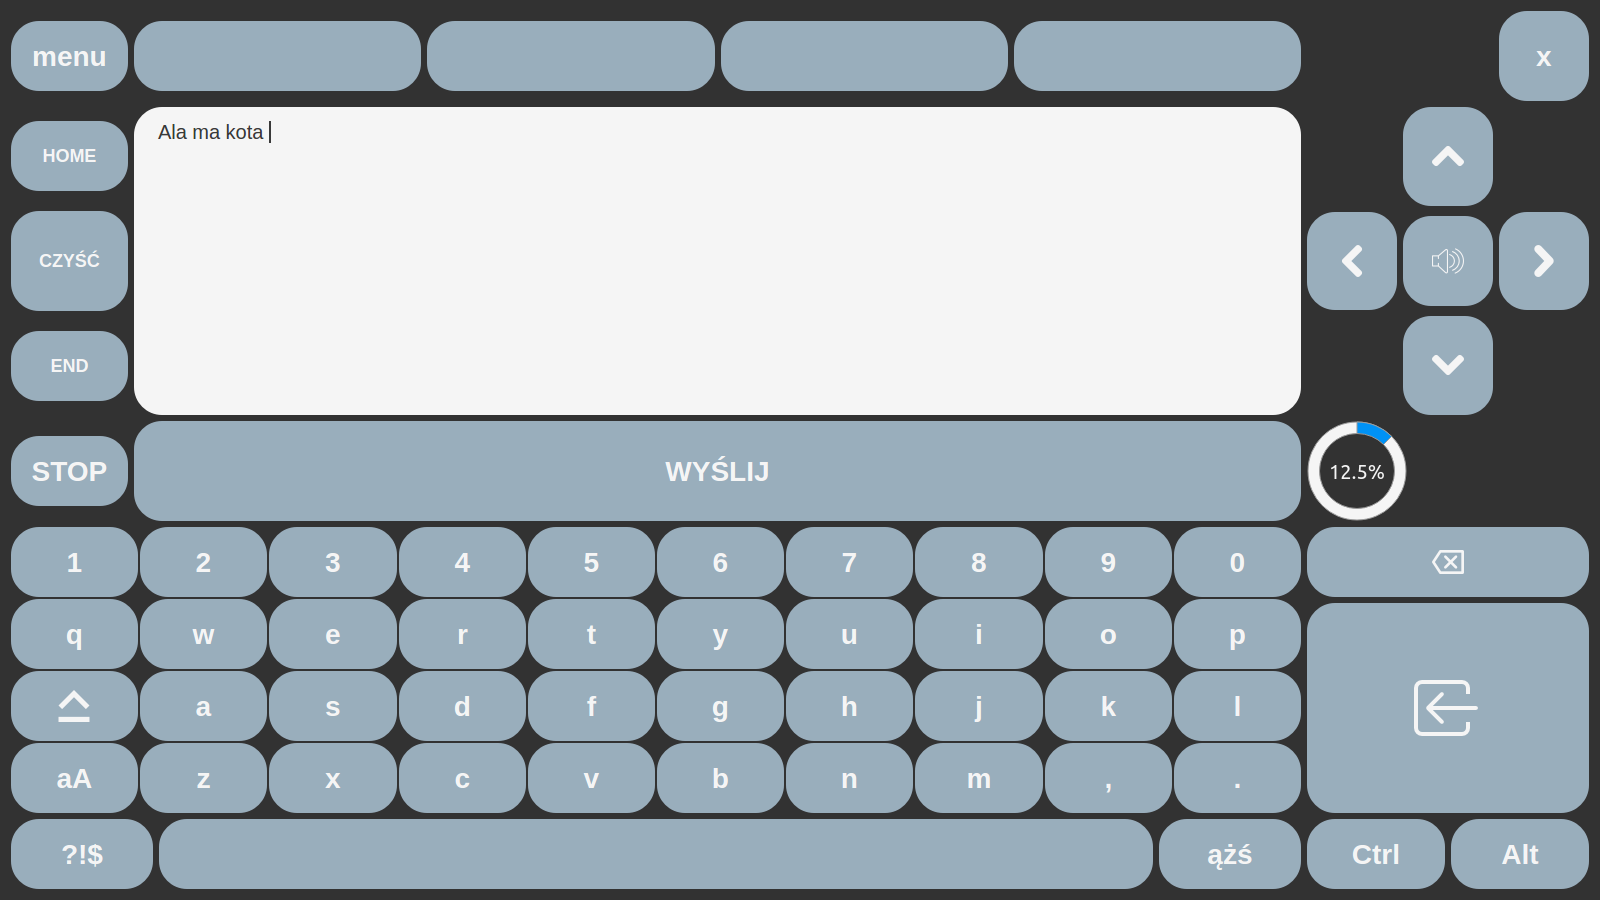
\includegraphics[width=1\textwidth]{img/added.jpg}}
		\caption{Tekst i podpowiedzi po wybraniu sugerowanego tekstu. }
		\label{fig:textAuto}
\end{figure}
\section{Projekt testów}


\section{Cele biznesowe}
\subsection{Możliwość dalszego rozwoju}
\section{Wymagania pozafunkcjonalne}

\subsection{Ergonomia}
\subsection{Ograniczenia}
\section{Podsumowanie}


\end{document}